\documentclass{article}

\usepackage{amsmath}
\usepackage{amsthm}
\usepackage[utf8]{inputenc}
\usepackage[portuguese]{babel}
\usepackage{graphicx}

\usepackage{pgffor}

\title{Currículo para Afterschool de Análise Real}
\author{}
\date{}

\newtheorem{prop}{Prop}

\addto\captionsportuguese{
	\renewcommand{\proofname}{Dem}
}

\begin{document}
	\maketitle
	
	\section{Metodologia}
	
	Esta iteração de uma Afterschool de Análise Real funcionaria em regime de `clube'. Isto é, aos alunos (algures entre 15 e 20, do 9º ao 12º ano) seria providenciado material de estudo (se possível, uma cópia do livro \emph{Introdução à Análise Matemática} do J. C. Ferreira), um local de discussão (um servidor de Discord?), um local de encontro (encontros semanais) e apoio de orientadores durante estes encontros. A ideia é que os alunos estudem o material por si mesmos, e os encontros servem para estimular a discussão e entreajuda.
	
	A primeira iteração teria uma duração curta para fazer a experiência, algures entre 6 e 8 semanas. Cada sessão teria aproximadamente o seguinte formato: (Muito sujeito a mudança, obviamente)
	
	\begin{itemize}
	\item Duração de 2h com uma pausa no meio
	
	\item Iniciar com apresentação de exercícios novos para iniciar e incentivar discussão
	
	\item De resto, deixar os alunos conviver, com intervenção mínima dos orientadores, exceto para resolver possíveis dúvidas.
	\end{itemize}
	
	O progresso dos alunos será, em princípio, assíncrono. Isto requer então alguns cuidados. Por exemplo, os exercícios apresentados terão que ser dados em vários `patamares', para qualquer aluno de qualquer nível ter algo em que pensar.
	
	De facto, o currículo será dividido em níveis, cada um destes uma quantidade pequena de matéria, digerível em mais ou menos uma hora de trabalho. Por exemplo, a prova de ingresso (ver abaixo) corresponderá ao nível 1. Cada aluno terá um nível associado. Este nível será maioritariamente usado pelos orientadores para determinar que tipo de exercícios dar no início de uma sessão. Um aluno começará no nível 1 (em princípio, um aluno que entre já `passou' a prova de ingresso, que o qualifica como nível 1).
	
	Para passar de um nível para o outro, vejo duas possibilidades. Estou de momento indeciso sobre qual delas será melhor:
	
	\begin{itemize}
	\item Autoavaliação.
	
	Pros:
	\begin{itemize}
	\item Menos trabalho da parte dos orientadores
	
	\item Os alunos haverão de saber melhor o que sabem do que nós
	\end{itemize}
	
	Contras:
	\begin{itemize}
	\item Possibilidade de um aluno se auto-reportar como sabendo coisas que não entende realmente, sem saber que não as entende
	\end{itemize}
	
	\item Subir por cumprir um certo requerimento, e.g. um teste ou uma `prova oral' com um orientador.
	
	Pros:
	\begin{itemize}
	\item É mais difícil um aluno chegar a um nível sem entender bem os níveis anteriores
	
	\item Dá alvos concretos e tangíveis aos alunos
	\end{itemize}
	
	Contras:
	\begin{itemize}
	\item Mais trabalho para os orientadores
	
	\item Há o perigo de entender mal um aluno e não subir quem mereça. Isto pode afetar autoestima e motivação.
	\end{itemize}
	\end{itemize}
	
	\section{Prova de ingresso}
	
	Para a prova de ingresso, é esperado que um aluno leia as seguinte páginas. (As fotos serão substituídas por scans mais legíveis.)
	
	\foreach \n in {1,...,7}{
		\includegraphics[width=\linewidth]{pg\n}
		\newpage
	}
	
	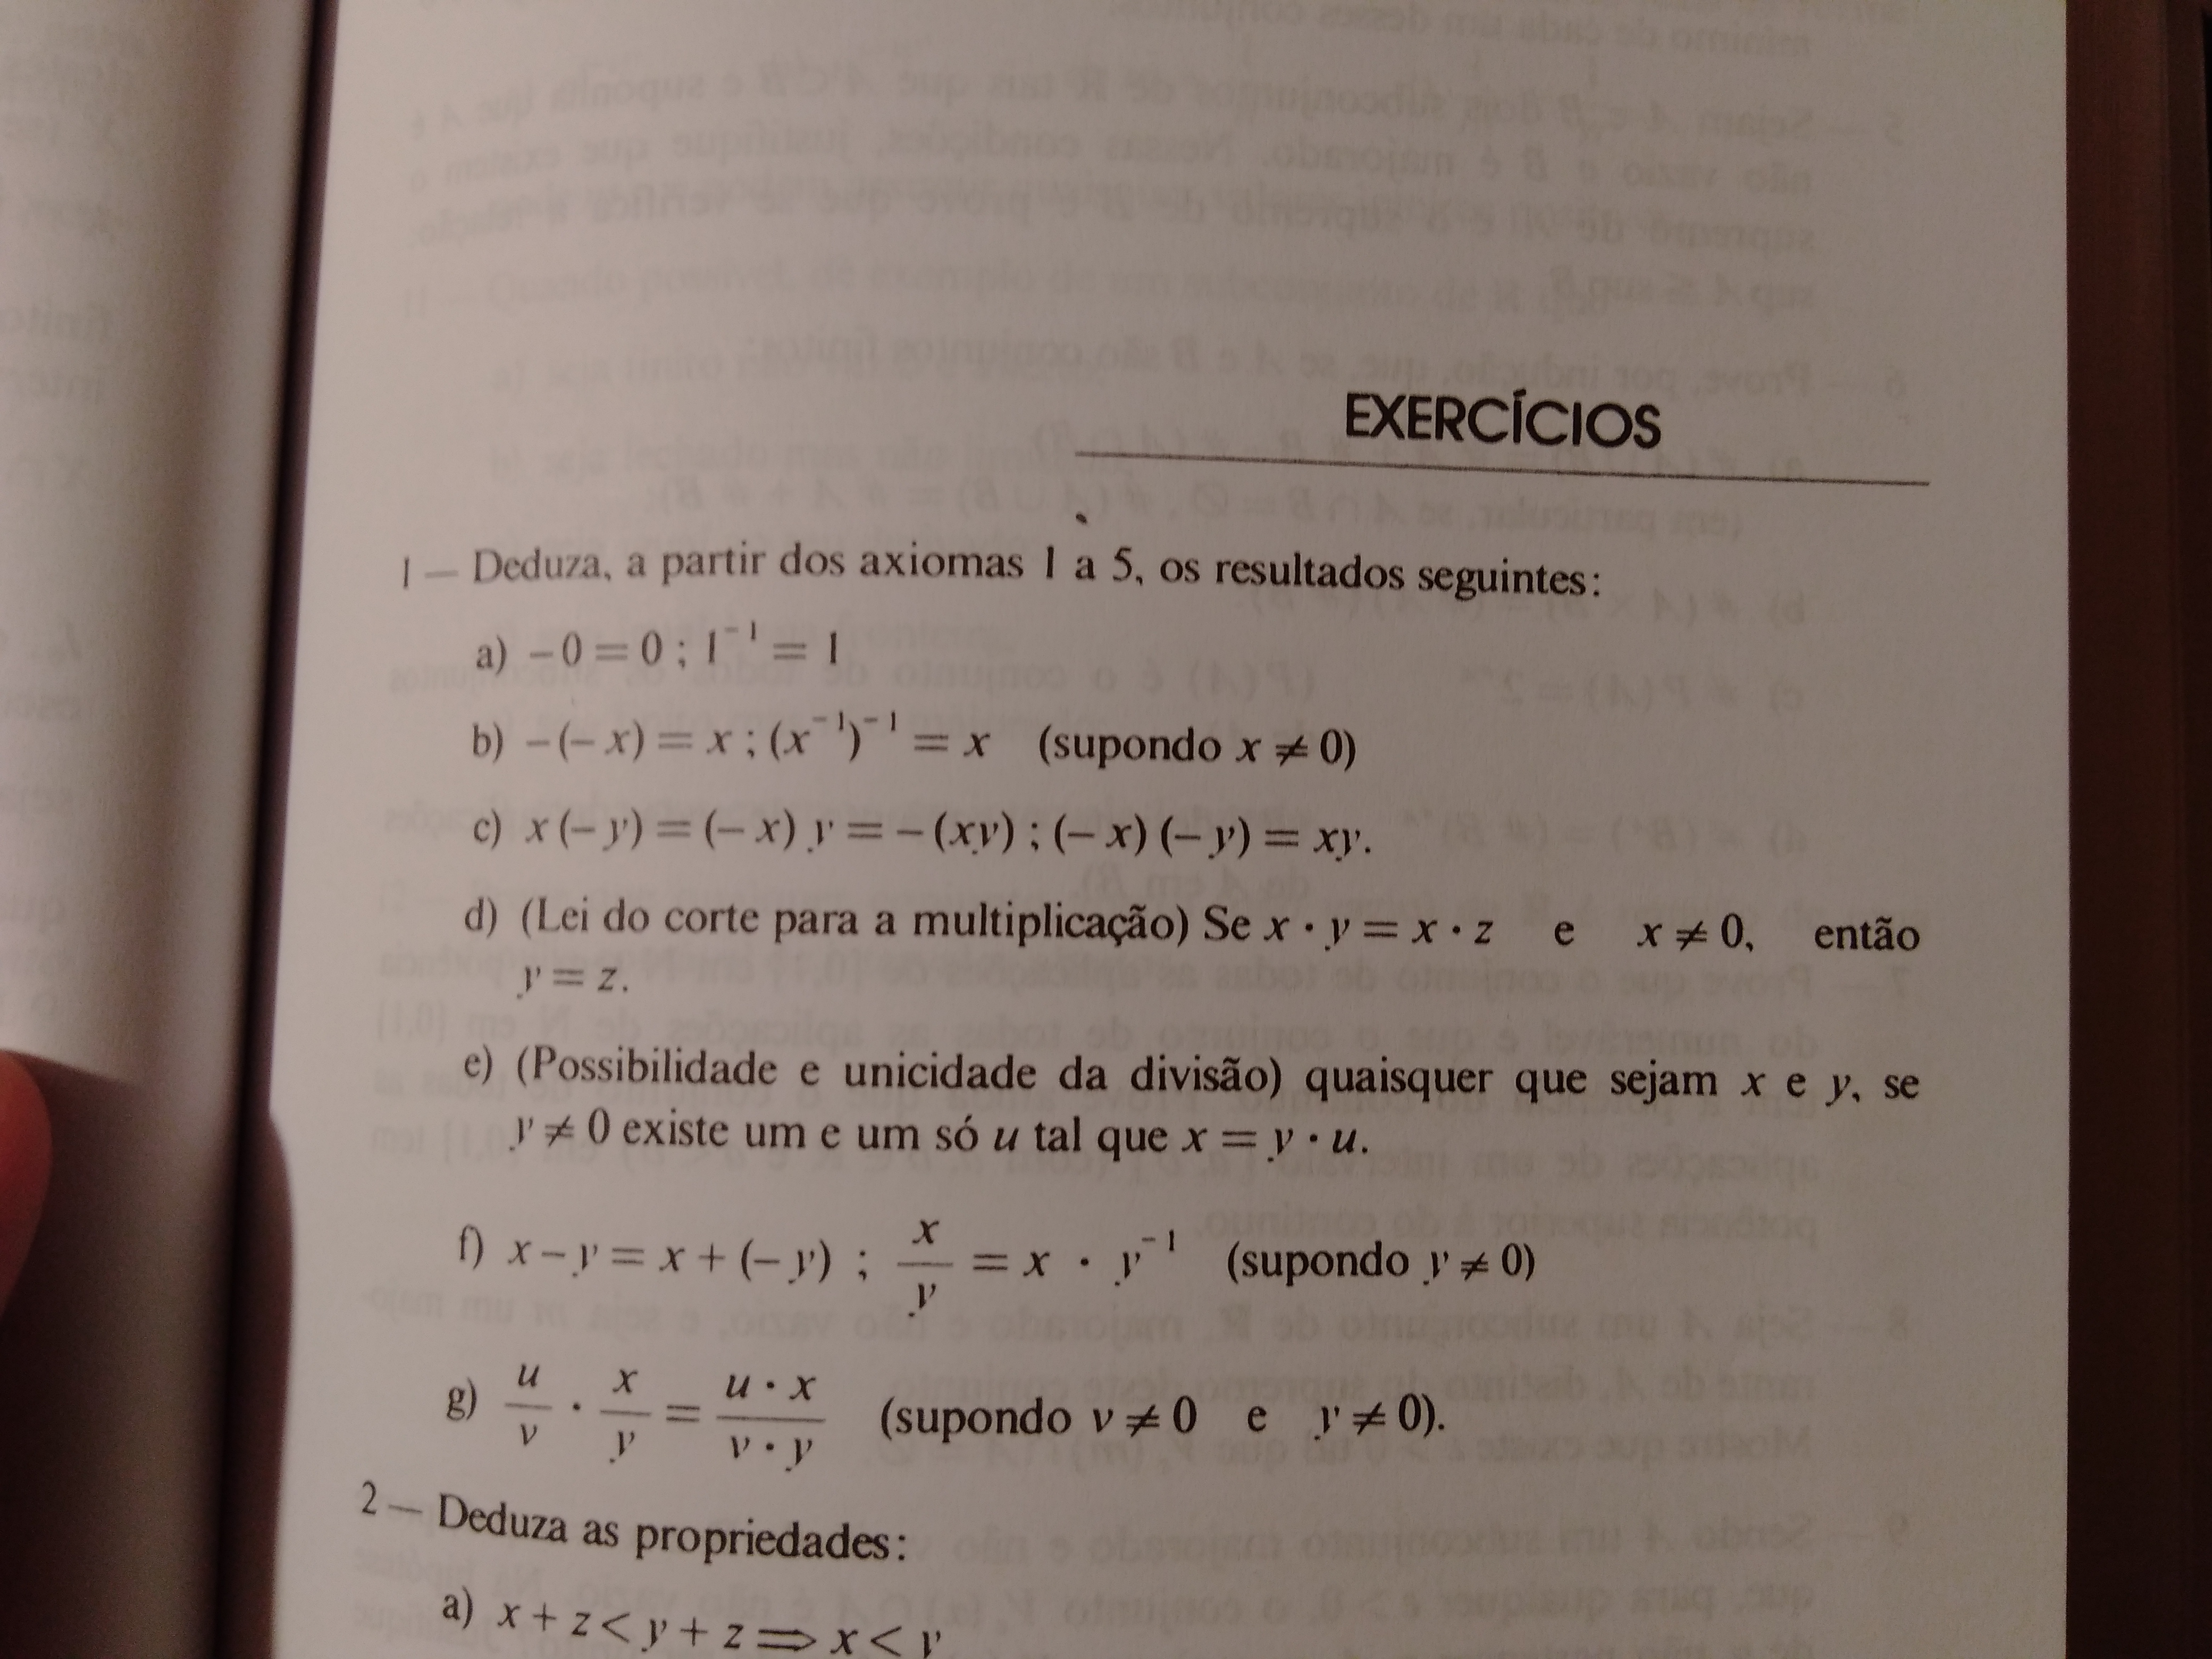
\includegraphics[width=\linewidth]{ex1}
	\newpage
	
	Solicita-se que os alunos submetam um ou mais dos seguintes, como prova de ingresso:
	
	\begin{itemize}
	\item Solução parcial ou total do exercício 1, acima
	
	\item Resumo do capítulo acima, completo com demonstrações. Preferível se as demonstrações forem pelas palavras próprias do aluno. Pontos extra por demonstrações que não são apenas as demonstrações do livro escritas por outras palavras.
	
	\item Qualquer outra coisa que o aluno deseje submeter, desde que mostre uma capacidade de interpretar, pensar e demonstrar coisas.
	\end{itemize}
	
	\section{Níveis}
	
	A seguinte enumeração dos níveis está organizada da forma:\\
	Número. Parágrafo associado; Exercício associado.
	
	Para um aluno completar um nível, e esperado que leia o parágrafo respetivo e saiba resolver o exercício associado.
	
	Estão marcados alguns níveis com asteriscos. Estes são níveis que talvez mereçam alguma revisão, visto que o seu conteúdo poderá ser particularmente difícil e os alunos talvez careçam de contexto para os conceitos introduzidos.
	
	\begin{enumerate}
	\item I.1.1 Axiomas de um corpo; Ex 1
	
	\item I.1.2 Axiomas de ordem; Ex2
	
	\item I.1.3 Números naturais, inteiros e racionais; Ex3 *
	
	\item I.1.4 e I.1.5, Axioma do supremo; Ex4 e Ex5
	
	\item I.1.6 Cardinalidades; Ex6 e Ex7
	
	\item I.2.1, I.2.2, I.2.3 Conceitos topológicos; Ex8 até Ex11
	
	(Exercício bónus: Ex12)
	
	\item II.1.1 Sucessões; Ex1
	
	\item II.1.2 Limite; Ex2 e Ex3
	
	\item II.1.3 Sucessões limitadas e sucessões de Cauchy; Ex4
	
	\item II.1.4 A reta acabada; (Por determinar)
	
	\item II.1.5 (Primeira metade) Algumas operações com limites; Notação `O-grande' e `o-pequeno'; Ex5
	
	\item II.1.6 (Segunda metade) Exponenciais reais; (Por determinar)
	
	(Exercícios bónus: Ex6 até Ex11)
	\end{enumerate}

\end{document}